\renewcommand{\MayorVer}{1}
\renewcommand{\MenorVer}{0}
\renewcommand{\Codigo}{G-1-PRO}
\renewcommand{\FechaPub}{2023--01}
\renewcommand{\Titulo}{Programa de verificación y actualización de información documentada}

\section{\Titulo}
\label{informacion.actualizacion}
\index{Procedimiento!programa de verificación y actualización dea}
\index{Información documentada!programa de verificación y actualización de}

\subsection{Objetivos}
\index{Información documentada!objetivos}
\begin{itemize}
    \item \textbf{Establecer} un programa para la validación de la \gls{informacion-documentada} que maneja \GLS{RDF};
    \item \textbf{Procurar} que se validen los requisitos de cada programa establecido y con base en los nuevos requerimientos, se actualicen los mismos;
    \item \textbf{Proponer} fechas para la actualización de revisiones mayores y menores.
\end{itemize}

\subsection{Alcance}
\index{Información documentada!alcance}
\begin{itemize}
    \item Este procedimiento va dirigido al área operativa encargada de la modificación de la \gls{informacion-documentada} y de los \gls{PPR} y \gls{PPRO} establecidos por \GLS{RDF};
    \item el alcance de la validación y revisión de la información contempla, pero no está limitada a:
          \begin{itemize}
              \item comunicaciones externas o internas;
              \item especificación de servicios;
              \item formularios;
              \item listas de verificación;
              \item listas;
              \item mapas de proceso;
              \item organigramas;
              \item planes;
              \item políticas;
              \item procedimientos;
              \item instrucciones de trabajo;
              \item programas.
          \end{itemize}
\end{itemize}

\subsection{Terminología y definiciones}
\begin{description}
    \defglo{PPR}
    \defglo{PPRO}
    \defglo{validacion-documental}
    \defglo{revision-documental}
    \defglo{informacion-documentada}
\end{description}

\subsection{Procedimiento}
\index{Información documentada!procedimiento}
\begin{figure}[htb]
    \centering
    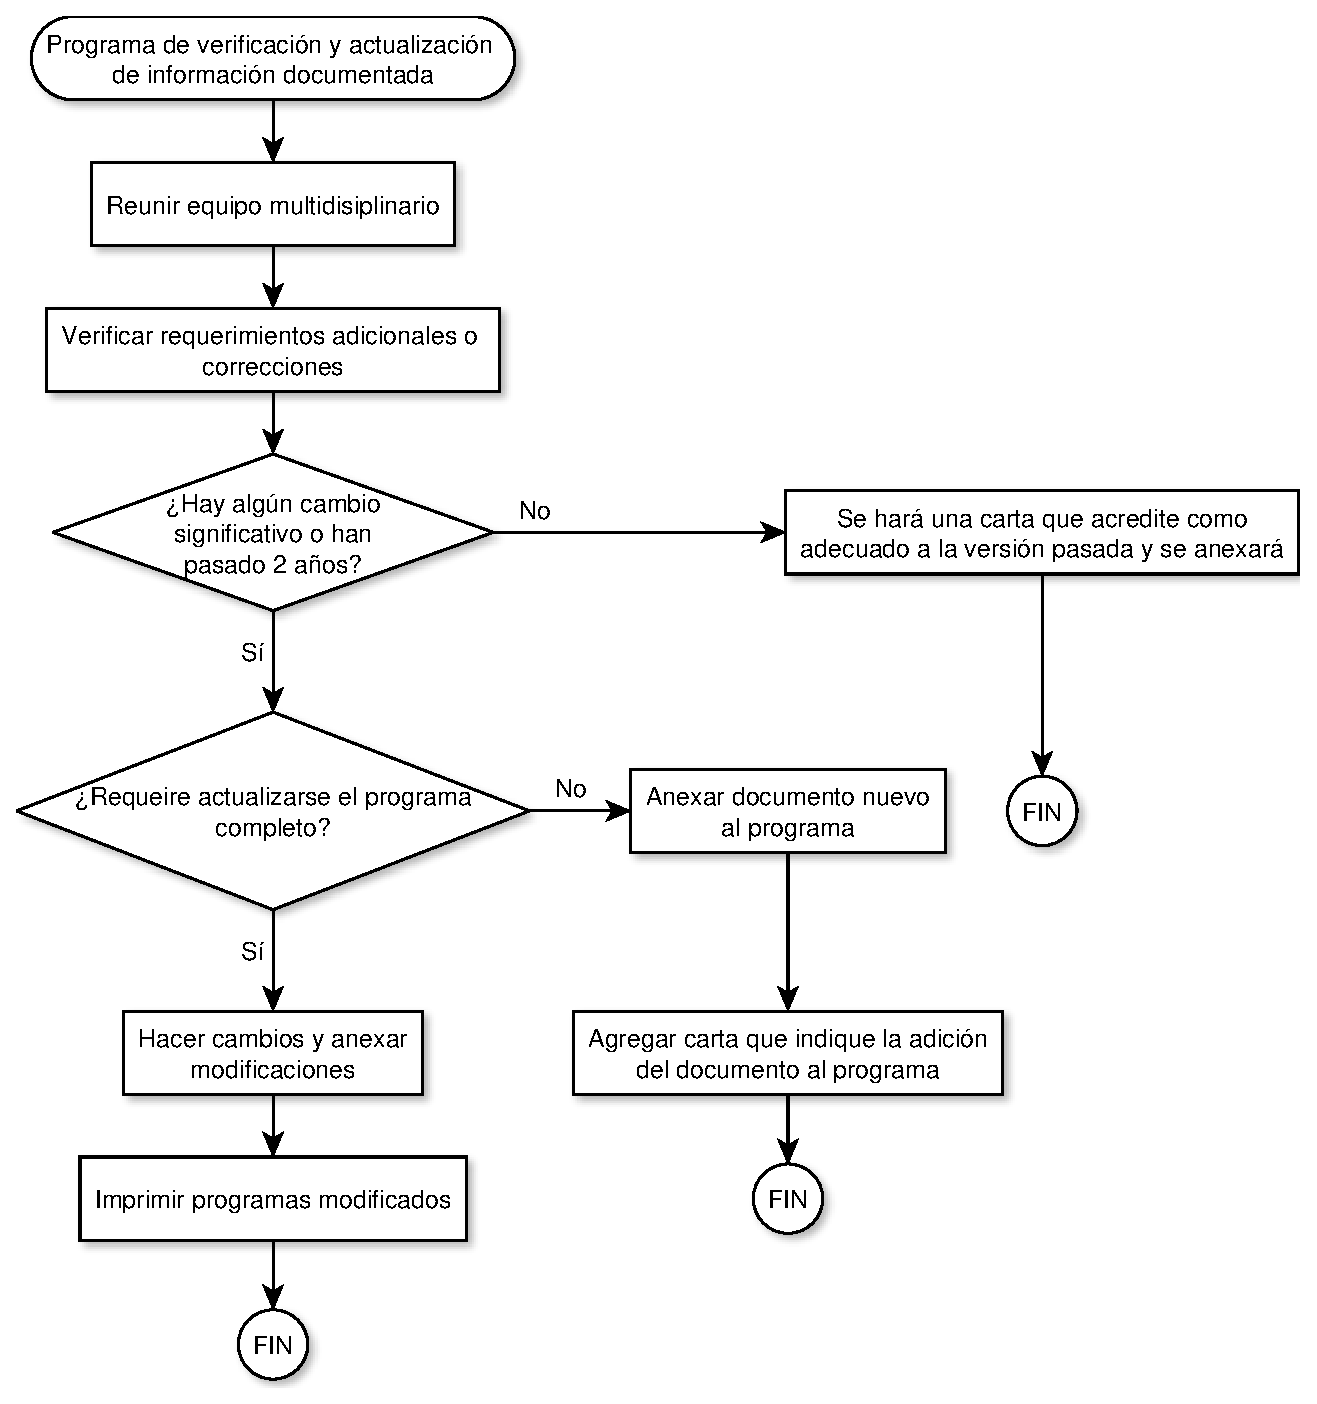
\includegraphics[width=0.5\linewidth]{src/diagramas/G1_AV1.eps}
    \caption{Diagrama de flujo del proceso para verificar y/o actualizar \gls{informacion-documentada}.}
\end{figure}

\subsubsection{Revisión de la información documentada}
\index{Información documentada!revisión}
\label{documentacion:revision}
\begin{itemize}
\item Se tienen que evaluar anualmente los programas de \GLS{RDF} con el propósito de determinar áreas de oportunidad. Esto tiene que hacerse con ayuda de un equipo multidisciplinar constituido por administradores de las áreas operativas pertinentes a la \gls{informacion-documentada} que se va a validar;
\item en caso de que se considere adecuada la información establecida en la \gls{informacion-documentada} analizada, se hará una carta que acredite como vigente el programa (ver \cref{documentacion:validacion}).
\end{itemize}

\subsubsection{Validación de la información documental}
\index{Información documentada!validación}
\label{documentacion:validacion}
Una vez revisada la información documental de los programas pertinentes, si se acuerda que la información contenida sigue vigente se tiene que hacer el siguiente procedimiento:
\begin{itemize}
    \item Revisar programas e \gls{informacion-documentada} asociada con ayuda de un equipo multidisciplinar;
    \item elaborar una carta membretada que acredite como \emph{vigente} el programa y se establezca una fecha de revisión futura;
    \item se debe de firmar la carta por el gerente de almacén y por el jefe de aseguramiento de calidad;
    \item en caso de que se tenga que hacer algún \textit{addendum} que no involucre una reestructuración completa del contenido o de la serialización de los documentos; él ---o los--- documentos nuevos deberán agregarse a la carpeta del programa al que pertenece y se agregará una carta membretada que documente las modificaciones o \textit{addendums} al programa. Esta carta debe de firmarse por el gerente de almacén y por el jefe de aseguramiento de calidad.
\end{itemize}

\subsubsection{Formación del equipo multidisciplinar}
\index{Información documentada!equipo multidisciplinar, formación de}
\label{documentacion:formacionEquipo}
La función de tener una reunión con un \emph{equipo multidisciplinar} es el poder determinar que carencias existen en los programas que cada área operativa utiliza.

Para la formación del equipo se debe de considerar lo siguiente:
\begin{itemize}
    \item No es necesario mantener una lista del equipo multidisciplinar estática;
    \item no se requiere forzosamente que se parte del equipo el jefe de cada área, puede pertenecer a la junta cualquier empleado del área operativa;
    \item se tiene que definir el alcance de la junta y el tiempo que se dedicará;
    \item pueden conducirse entrevistas para determinar carencias en el SGC.
    \item no se requiere documentar la minuta de esta reunión, pero sí se requiere elaborar la \emph{carta de vigencia de programa} (ver \cref{documentacion:validacion,carta.validación}).
\end{itemize}


\subsection{Frecuencia}
\index{Información documentada!frecuencia de revisión y validación}

\begin{table}[h]
    \centering
\begin{talltblr}[%
        caption = {Frecuencia de los procesos asociados con la actualización de \gls{informacion-documentada}.},
        label = {freq.act},
        note{$\dag$} = {Puede ser, por ejemplo, la inclusión de un nuevo formulario, procedimiento, instrucción de trabajo, ayuda visual, etc\dots}
        ]
        {%
        colspec = {X[c]X[c]},
        width = 0.6\linewidth,
        rowhead = 1
        }
        \toprule
        Proceso                                                  & Frecuencia                                                                                          \\
        \midrule
        Validación de la \gls{informacion-documentada}                 & Anualmente                                                                                          \\
        Actualización completa de la \gls{informacion-documentada}     & Cada que se haga un cambió considerable o cuando existan cambios en la estructura de los documentos \\
        Generación de carta aprobativa de información documental & Cada que se tenga que hacer un addendum minúsculo a un programa\TblrNote{$\dag$}                    \\
        \bottomrule
\end{talltblr}
\end{table}

\subsection{Responsabilidades}
\index{Información documentada!responsabilidades}
\begin{itemize}
    \item \textbf{Aseguramiento de calidad:} se encarga de producir los cambios al programa;
    \item \textbf{Equipo multidisciplinar:} se encargará de determinar los cambios y adiciones a los programas establecidos;
    \item \textbf{Gerente de almacén:} verificación de las modificaciones y aprobación.
\end{itemize}

\subsection{Acciones preventivas}
\index{Información documentada!acciones preventivas}
\begin{itemize}
    \item Se coordinará con el \emph{equipo multidisciplinar} una fecha para la junta con anticipación suficiente.
\end{itemize}

\subsection{Acciones inmediatas}
\index{Información documentada!acciones inmediatas}
En caso de que no se haya conducido la actualización completa o la verificación de la información documental no será requerido elaborar un estudio de causa raíz, ya que esto no se considera un problema a la inocuidad de los alimentos, sin embargo se procederá a hacer las siguientes acciones inmediatas.

\subsubsection*{En caso de que la junta no se pudiera acordar}
\index{Información documentada!acciones inmediatas!junta no concretada}
\begin{itemize}
    \item Se coordinará con el \emph{equipo multidisciplinar} una fecha diferente para la junta con anticipación suficiente.
\end{itemize}

\subsubsection*{En caso de que las actualizaciones no se hayan concretado en el periodo establecido}
\index{Información documentada!acciones inmediatas!actualización en proceso}
\begin{itemize}
    \item Se seguirá utilizado la \gls{informacion-documentada} anterior hasta que se logren publicar las modificaciones.
\end{itemize}

\begin{changelog}[simple, sectioncmd=\subsection*,label=changelog-1.0]
    \begin{version}[v=1.0, date=2023--01, author=Pablo E. Alanis]
        \item Primera edición.
    \end{version}
\end{changelog}